\documentclass{standalone}
\usepackage{pgfplots,siunitx}
\usetikzlibrary{shadings,decorations.pathmorphing,arrows.meta,patterns}
\pgfplotsset{
    compat=1.18,
    reg/.append style={
        xmin =-4.5,
        xmax =4.5,
        ymin =-4.5,
        ymax = 4.5,
        axis lines = center,
        xtick = {-4,...,4},
        ytick = {-4,...,4},
        height = 6cm,
        width = 6cm,
        grid = major,
        grid style = {thick, dotted},
        tick label style = {font=\small}
      },
    myplot/.append style={
      smooth,domain=-4:4,samples=50,thick
    },
    wave/.style={
      width=5cm,
      height=5mm,
      scale only axis,
      ultra thick,
      xmin=0,
      xmax=10,
      hide axis
    }
  }

\begin{document}
  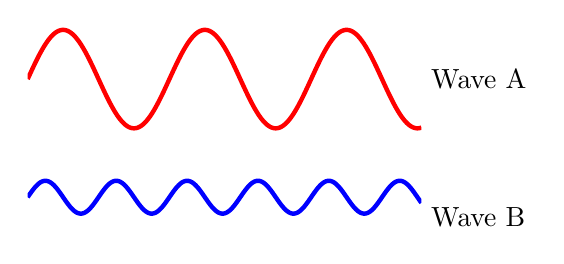
\begin{tikzpicture}
    \begin{scope}
      \node[anchor=west] at (5,0.75) {Wave A};
      \begin{axis}[red,wave,height=15mm] 
        \addplot[domain=0:10,samples=900]{sin(100*x)};
      \end{axis}
    \end{scope}

    \begin{scope}[shift={(0,-1)}]
      \node[anchor=west] at (5,0) {Wave B};
      \begin{axis}[blue,wave] 
        \addplot[domain=0:10,samples=900]{sin(200*x)};
      \end{axis}
    \end{scope}
  \end{tikzpicture}
\end{document}